\documentclass{training}
\schoollogo{../../resources/intros/UX-02-lets-fight-harassment.jpg}
\newcommand{\uxfond}{../../resources/fond/UX-02-lets-fight-harassment.png}
% Filigrane PAR MODULE : \uxfond (PNG A4 dilue 30 %). Cadre noir vectoriel commun.
% Proportions original 744 px : marge 20/744, trait 1/744. Exterieur BLANC.
% Cadre via eso-pic +\put (coordonnees absolues) — pas de remember picture (decalage).
\usepackage{eso-pic}

\providecommand{\uxfond}{../../resources/fond/norme_fond_paliers_30.png}

\newlength{\uxmargin}
\newlength{\uxthick}
\newlength{\uxinnerw}
\newlength{\uxinnerh}
\setlength{\uxmargin}{0.02688\paperwidth}% 20/744
\setlength{\uxthick}{0.001344\paperwidth}% 1/744
\setlength{\uxinnerw}{\dimexpr\paperwidth-2\uxmargin-2\uxthick\relax}
\setlength{\uxinnerh}{\dimexpr\paperheight-2\uxmargin-2\uxthick\relax}

% Contenu strictement a l'interieur du trait (+ jour confortable).
\geometry{%
  includeheadfoot,
  left=22mm,
  right=22mm,
  top=20mm,
  bottom=18mm,
  headheight=30pt,
  headsep=5mm,
  footskip=12mm%
}

\AddToShipoutPictureBG{%
  \AtPageLowerLeft{%
    % Fond blanc page entiere
    \put(0,0){\color{white}\rule{\paperwidth}{\paperheight}}%
    % Filigrane module a l'interieur du cadre
    \put(\LenToUnit{\dimexpr\uxmargin+\uxthick\relax},\LenToUnit{\dimexpr\uxmargin+\uxthick\relax}){%
      \includegraphics[width=\uxinnerw,height=\uxinnerh]{\uxfond}}%
    % Cadre noir : bas, haut, gauche, droite
    \put(\LenToUnit{\uxmargin},\LenToUnit{\uxmargin}){%
      \color{black}\rule{\dimexpr\paperwidth-2\uxmargin\relax}{\uxthick}}%
    \put(\LenToUnit{\uxmargin},\LenToUnit{\dimexpr\paperheight-\uxmargin-\uxthick\relax}){%
      \color{black}\rule{\dimexpr\paperwidth-2\uxmargin\relax}{\uxthick}}%
    \put(\LenToUnit{\uxmargin},\LenToUnit{\uxmargin}){%
      \color{black}\rule{\uxthick}{\dimexpr\paperheight-2\uxmargin\relax}}%
    \put(\LenToUnit{\dimexpr\paperwidth-\uxmargin-\uxthick\relax},\LenToUnit{\uxmargin}){%
      \color{black}\rule{\uxthick}{\dimexpr\paperheight-2\uxmargin\relax}}%
  }%
}

\makeatletter
\fancyhf{}
\fancyheadoffset{0pt}
\renewcommand{\headrulewidth}{0pt}
\lhead{\parbox[t]{0.56\textwidth}{\RaggedRight\footnotesize\sloppy\@title}}
\rhead{\parbox[t]{0.36\textwidth}{\RaggedLeft\footnotesize\sloppy\@subtitle}}
\cfoot{\thepage}
% Coupures : underscore et slash dans les noms de fichiers / consignes
\DeclareRobustCommand{\_}{\textunderscore\allowbreak}
\makeatother

% Evite les depassements de longues lignes (Github, Name_FirstName_...)
\sloppy
\emergencystretch=3em
\hbadness=10000

% Sommaire type 42 : chapitres seulement
\setcounter{tocdepth}{0}
\renewcommand{\cftchappresnum}{}
\renewcommand{\cftchapaftersnum}{}
\setlength{\cftchapnumwidth}{2.0em}
\setlength{\cftbeforechapskip}{0.35em}
\cftsetindents{chapter}{0em}{2.0em}


\begin{document}

\title{Let's fight harassment}
\subtitle{Piscine UX/UI --- UX}
\member{Piscine UX/UI}{https://github.com/01-edu/UX-UI}
\summary{Research and a public message. The brief is not a script.}
\version{1.0}
\prerequisite{The previous module of this piscine, or none if this is your first.}
\maketitle

\newpage
\tableofcontents
\newpage


\chapter{Instructions}

The foreword is not an exercise. It will not be graded. The exercises start at the next chapter, from the easiest contract to the hardest. A later exercise is not taken into account if an earlier one does not hold.

Only what is in the turn-in directory of an exercise is looked at. Do not add files that the exercise does not name. The name of a deliverable follows the pattern in the exercise: \texttt{Name\_FirstName\_DeliverableName\_Date\_VersionNumber}.

You will not be given the gesture. The examples in an exercise sometimes carry a constraint that the sentence does not repeat. Read them. Your other references are the manual of the tool you picked, the person sitting next to you, and the links printed in the exercise.

The order is the order of the quest. Skipping a step because a later screen looks more interesting produces a screen nobody can explain.

\subsection*{About the pictures}

The mark on the cover is the picture of this module. The pale steps behind the text are the page ground. Neither one is a hint.

\subsection*{About machines that write}

You may use a tool to look up a term, the way you would use a dictionary. You may not replace an interview, a test, or a file with a generated text and sign it. If you cannot point at the person, the screen, or the line you claim, the exercise is not done.


\chapter{Foreword}

A poster is a sentence a street can read. A.~M.~Cassandre treated the poster as a public voice, not as a decoration (see the posters gathered by the MoMA, \url{https://www.moma.org/artists/1015}). This quest asks for that kind of voice: a message aimed at a real audience. It does not ask you to depict harm, and it does not hand you the message.

\begin{center}
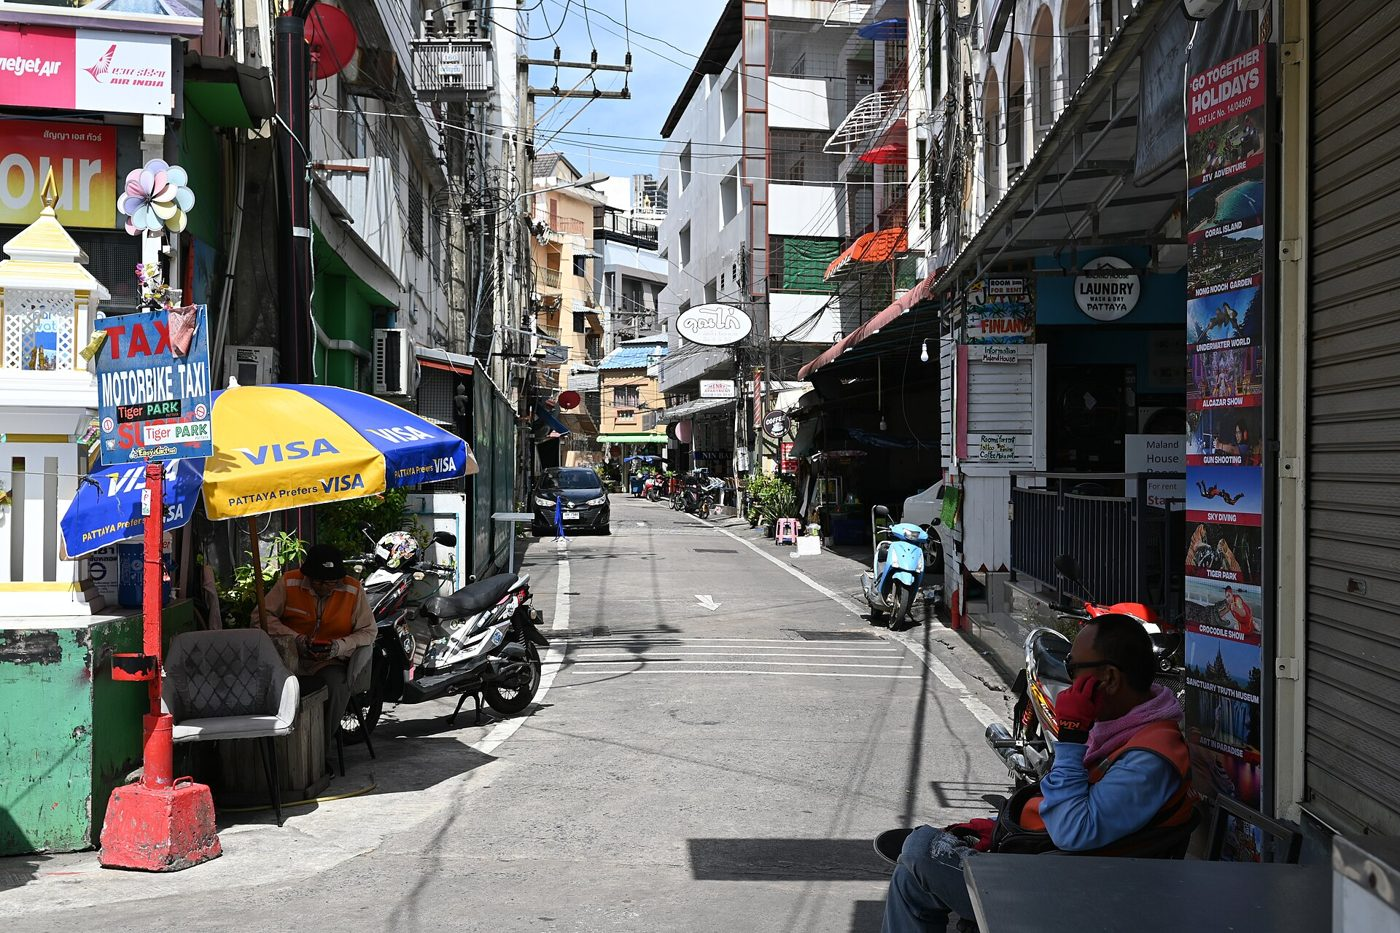
\includegraphics[width=0.78\textwidth,height=0.32\textheight,keepaspectratio]{../../resources/intros/UX-02-lets-fight-harassment.jpg}\\[0.4em]
{\footnotesize Picture: PattayaPatrol, CC BY-SA 4.0}
\end{center}

Recommended watching. The videos are context. They are not the deliverable.
\begin{itemize}
\item UX - Introduction \& Quest n°1, 01Edu \url{https://www.youtube.com/watch?v=UbE6WMeuvQg&list=PLHyAJ_GrRtf-RAtfngbRrFh1XDTnyXFDe}
\end{itemize}

\chapter{Exercise 00: UX III - Ex 1 - Competitive Analysis}
\exnumber{00}
\extitle{UX III - Ex 1 - Competitive Analysis}
\exfiles{ex00/zip archive, named Name\_FirstName\_DeliverableName\_Date\_VersionNumber}
\exauthorize{Those named in the exercise}
\makeheaderfiles

\textbf{Context:}

Quest n°3 is about Empathy.

In this scenario, the principal of your high school heard you were a designer. They chose to reach you to help them face school harassment among teenagers.

School harassment describes school-based harassment behaviors. It is characterized by the repeated use of violence, including mockery and other humiliations.

As a matter of fact, they realized they didn't know this generation (15 to 18-year-olds) very well. So they are asking you to conduct user research to meet this population and understand them.

Your job is to explore your topic and use various tools included in this "Empathize" phase.

\textbf{Instructions:}

Conduct a competitive analysis among 10 associations or organizations fighting school harassment.

You can pick 10 organizations worldwide, or from your home region or home country. Let's browse!

Compare these 10 organizations' main actions, channels, values, according to the criteria you assume are relevant.

\textbf{Deliverables :}

\begin{itemize}
\item A competitive report with an introduction that explains your main conclusions (PDF)
\item A chart to show the competitive landscape, with 2 axes of your choice (digital, psychological, local, closeness to students, institutional, etc.) (PDF)
\item A table to compare the organizations on 5 to 10 criteria (PDF)
\item Upload the documents on Github, in a zip folder named "ProjectTitle\_Name\_FirstName", with all project deliverables as follows: "Name\_FirstName\_DeliverableName\_Date\_VersionNumber".  For example, the first deliverable can be named as "Doe\_John\_MidFiPrototype\_05242024\_V1".
\item Add a title within all written documents.
\item Pay attention to the global aspect of the deliverables. They must be clear, simple and easy to read. You can get inspiration on canva.com but don't overload your design with too much details!
\end{itemize}

Resources:

\begin{itemize}
\item Competitive Analysis: How to approach it effectively \url{https://uxdesign.cc/competitive-analysis-how-to-approach-it-effectively-def97d130d2c}
\item Competitive Analysis Templates \url{https://venngage.com/blog/competitor-analysis-template/}
\end{itemize}

\textbf{Quote :}

\begin{itemize}
\item 'Always design a thing in its larger context: a chair in a room, a room in a house, a house in an environment, an environment in a city plan' Eero Sarrinen | Knoll
\item Creating a great design isn't just about understanding what the user wants. It's also about understanding and delivering on what the business needs.
\end{itemize}


\chapter{Exercise 01: UX III - EX 2 - Surveys}
\exnumber{01}
\extitle{UX III - EX 2 - Surveys}
\exfiles{ex01/PDF, named Name\_FirstName\_DeliverableName\_Date\_VersionNumber}
\exauthorize{Those named in the exercise}
\makeheaderfiles

\textbf{Instructions:}

Prepare a survey to gather quantitative data from your users.

And remember, you are not your user!

To be used in proper studies and get viable results, a form should gather at least 100 answers. The answers should give you countable data you can use to prove a point and confirm trends, not verbatims or details.

\textbf{Deliverables:}

\begin{itemize}
\item A PDF document including your objective(s) and your hypotheses, the questions, an introduction and a conclusion.
\item In the document, add the link to a survey ready to be spread
\item Upload the PDF document on Github, labeled as follows: "Name\_FirstName\_DeliverableName\_Date\_VersionNumber". For example, it can be labeled as "Doe\_John\_MidFiPrototype\_05242024\_V1".
\item Add a title within the document.
\item Pay attention to the global aspect of the document. It must be clear, simple and easy to read. You can get inspiration on canva.com but don't overload your design with too much details!
\end{itemize}

\textbf{Tips:}

Here are the recommended steps :

1. Define your objective, what you are looking for when spreading your form to people. Usually, this has to do with figures, proportions, etc.
2. Write down 1 to 3 hypotheses you have regarding this topic, that you need to either confirm or disprove.
3. Pick 3 to 5 main topics you need to get information on.
4. For each topic, write 1 to 3 closed-ended questions. Remember, your user has to answer with a choice in a list of prepared answers or use the option "other" to write down the answer they can't find in the prepared list.
5. Write some screening questions to have a few pieces of demographics (age, job, location, etc.). This allows you to make sure the answers you get are from your target.
6. Structure your questions in a funnel: start with broad questions to focus on specific topics or situations. Remember to stay neutral in your tone to ket the user tell their own story. Try to focus on 10 main questions.
7. Write a greeting introduction, describing briefly (1) who you are and (2) what you are looking for. No need to say too much, but enough to provide a framework and the purpose of the form.
8. Write a conclusion to thank your user for their time, and prepare the next steps. Ex: ask to have this form spread to 3 people, etc.

\textbf{Mandatory: ask them if they would be available for an anonymous in-person interview (over the phone, in-person, through video chat: whatever they are more comfortable with) because you'll have to conduct at least 3 interviews further on.}

\textbf{Resources:}

\begin{itemize}
\item Lean Survey Canvas: How to use it \url{https://medium.com/think-big-work-smart/the-lean-survey-canvas-1b0a00cab200}
\item User surveys - How to survey your users \url{https://refiner.io/blog/user-surveys/}
\item Designing a great survey with 3 simple steps \url{https://uxdesign.cc/designing-a-great-survey-with-3-simple-steps-283abaa67ad6}
\item UX Surveys: a quick guide to get the most out of them \url{https://uxdesign.cc/ux-surveys-a-quick-guide-to-get-the-most-out-of-them-1889d136be6a}
\item Better research through surveys \url{https://uxmastery.com/better-user-research-through-surveys/}
\item The user experience of surveys \url{https://uxdesign.cc/the-user-experience-of-surveys-a5420c82604a}
\end{itemize}

\textbf{Tools:}

\begin{itemize}
\item Typeform \url{https://www.typeform.com/}
\item Google Forms \url{https://docs.google.com/forms/u/0/}
\end{itemize}

\textbf{Quotes:}

\begin{itemize}
\item "Surveys measure and categorize attitudes or collect self-reported data that can help track or discover important issues to address." Norman Nielsen Group
\item Surveys are not accurate in providing behavioural data because USERS OMIT STEPS IN THE MIDDLE AND MEMORIES ARE FAULTY.
\end{itemize}


\chapter{Exercise 02: UX III - Ex 3 - Broadcast strategy}
\exnumber{02}
\extitle{UX III - Ex 3 - Broadcast strategy}
\exfiles{ex02/zip archive, named Name\_FirstName\_DeliverableName\_Date\_VersionNumber}
\exauthorize{Those named in the exercise}
\makeheaderfiles

\textbf{Instructions:}

Define and run your broadcast strategy among teenagers (15-18 years old)

Even though a proper survey requires at least 100 answers, for this exercise we request you to get 40.

\textbf{Deliverables:}

\begin{itemize}
\item A PDF document gathering your strategy. Please include:
\begin{itemize}
\item Who you are targeting (remember, you can focus on your hometown as well as the whole planet)
\item A few ideas about how to reach them
\item The channels you intend to use - be specific and include the links to the groups, forums, pages, account you plan to reach
\item At least 2 different messages
\item A plan A, a plan B, a plan C
\end{itemize}
\item A document to express your main feedback after running your broadcast strategy: what worked best? have you encountered any difficulties? What were they? How did you overcome them?
\item Upload the documents on Github, in a zip folder named "ProjectTitle\_Name\_FirstName", with all project deliverables as follows: "Name\_FirstName\_DeliverableName\_Date\_VersionNumber".  For example, the first deliverable can be named as "Doe\_John\_MidFiPrototype\_05242024\_V1".
\item Add a title within all written documents.
\item Pay attention to the global aspect of the deliverables. They must be clear, simple and easy to read. You can get inspiration on canva.com but don't overload your design with too much details!
\end{itemize}

\textbf{Tips:}

In order to do so, you need to be creative and strategic!

\begin{itemize}
\item Who are you targeting? Teenagers, bullies, persecutor, witnesses, parents, teachers, people in the administration? From where?
\item How can you reach them? Through which channels? On which forums, groups, with which hashtags? Will you try to get them through influencers?
\item What words and what tone will you use?
\item How will you approach them? What message will you write?
\item What have you planned if they don't answer right away?
\end{itemize}

Once your strategy is prepared, run it!

\textbf{Resource:}

\begin{itemize}
\item How to get more survey responses \url{https://rafflepress.com/how-to-get-more-survey-responses/}
\end{itemize}


\chapter{Exercise 03: UX III - Ex 4 - Interviews}
\exnumber{03}
\extitle{UX III - Ex 4 - Interviews}
\exfiles{ex03/Figma file and PDF, named Name\_FirstName\_DeliverableName\_Date\_VersionNumber}
\exauthorize{Those named in the exercise}
\makeheaderfiles

\textbf{Instructions:}

\begin{itemize}
\item Create an interview guide
\item Conduct 3 interviews with teenagers
\end{itemize}

After knowing more about trends and "What" people do thanks to surveys, the main goal is to understand "why".

\textbf{Deliverables:}

\begin{itemize}
\item A PDF document with an interview guide
\item A PDF document with 3 scripts 
\item An affinity diagram from your interviews (PDF or digital, on Miro or Figma for example)
\item Upload the documents on Github, in a zip folder named "ProjectTitle\_Name\_FirstName", with all project deliverables as follows: "Name\_FirstName\_DeliverableName\_Date\_VersionNumber".  For example, the first deliverable can be named as "Doe\_John\_MidFiPrototype\_05242024\_V1".
\item Add a title within all written documents.
\item Pay attention to the global aspect of the deliverables. They must be clear, simple and easy to read. You can get inspiration on canva.com but don't overload your design with too much details!
\end{itemize}

\textbf{Resources:}

\begin{itemize}
\item Respondent - Tool to find users \url{https://www.respondent.io}
\item How to conduct user interviews \url{https://uxdesign.cc/how-to-conduct-user-interviews-fe4b8c34b0b7?sk=9625632a522a9309a91297191e668565}
\item How to design better products through user interviews \url{https://uxdesign.cc/how-to-design-better-products-through-user-interviews-4c5142bb1fc4}
\item Asking the right questions \url{https://uxdesign.cc/asking-the-right-questions-on-user-research-interviews-and-testing-427261742a67}
\end{itemize}

\textbf{Tips:}

Here are the recommended steps :

1. Define your objective, what you are looking for when interviewing people. Usually, this has to do with your user's habits, and the most painful problems they have regarding this topic.
2. Write down 1 to 3 hypotheses you have regarding this topic, that needs to be either confirmed or disproved.
3. Pick 3 to 5 main topics you need to get information on.
4. For each topic, write 1 to 3 open-ended questions. Remember, your user cannot answer with "Yes" or "No"! Ex: How, Why, What, When, Tell me about the last time you did... etc. If you really need to introduce a new topic by a close-ended question, ask why right after.
5. Write some screening questions to have a few pieces of demographics (age, job, location, etc.)
6. Structure your questions in a funnel: start with broad questions to focus on specific topics or situation. Remember to stay neutral in your tone to let the user tell their own story. Try to focus on 10 main questions.
7. Write a greeting introduction, describing briefly (1) who you are and (2) what you are looking for. No need to say too much, but enough to provide a framework and the purpose of the interview.
8. Write a conclusion to thank your user for their time, and prepare the next steps. Ex: ask to be put in touch with someone they know and who could be interested in this topic, etc.


\chapter{Exercise 04: UX III - Ex 5 - Personas}
\exnumber{04}
\extitle{UX III - Ex 5 - Personas}
\exfiles{ex04/Figma file and PDF, named Name\_FirstName\_DeliverableName\_Date\_VersionNumber}
\exauthorize{Those named in the exercise}
\makeheaderfiles

\textbf{Instructions:}

Let's create a persona based on your quantitative research and your interviews.

Your persona card should include common trends amongst the people you got data from (habits, verbatims, fears, drivers, frustration, and pain points).

Reminder: Your persona is fictional and should not have the exact name or picture as someone you interviewed, but remember a persona is here so you can make decisions as a designer.

\textbf{Deliverables:}

\begin{itemize}
\item A PDF persona card extracted from a Figma file
\item Upload the PDF document on Github, labeled as follows: "Name\_FirstName\_DeliverableName\_Date\_VersionNumber". For example, it can be labeled as "Doe\_John\_MidFiPrototype\_05242024\_V1".
\item Add a title within the document.
\item Pay attention to the global aspect of the document. It must be clear, simple and easy to read. You can get inspiration on canva.com but don't overload your design with too much details!
\end{itemize}

\textbf{Resources:}

\begin{itemize}
\item Make your persona great again \url{https://uxdesign.cc/personas-e60c1c06ead1}
\item Persona, journey maps, user flow, site map, OH MY! \url{https://uxdesign.cc/personas-journey-maps-site-maps-and-user-flows-oh-my-e71d044b4bcb}
\item Persona framework \url{https://miro.medium.com/max/1400/0*RbHfR6BHhhFIENNf}
\end{itemize}

\textbf{Quotes:}

\begin{itemize}
\item If you design for everyone, you delight no one.
\item A good user persona is the one based on user research, without regard to how many attributes we can describe.
\end{itemize}


\chapter{Exercise 05: UX III - Ex 6 - User Journey}
\exnumber{05}
\extitle{UX III - Ex 6 - User Journey}
\exfiles{ex05/Figma file, named Name\_FirstName\_DeliverableName\_Date\_VersionNumber}
\exauthorize{Those named in the exercise}
\makeheaderfiles

\textbf{Instructions:}

Now you have your persona, it's time to set it in motion.

Design a User Journey to represent your persona in their environment across the time, with key steps or actions related to our current topic (harassment).

The timeline can be of a day, a few hours, or a week. Please include the key moments related to harassment alongside the emotions related to each step. Use the material from your interviews and surveys.

Then, highlight the main pain points that need to be solved.

\textbf{Deliverable:}

\begin{itemize}
\item A Figma document with your persona's user journey
\item Upload the Figma file on Github, labeled as follows: "Name\_FirstName\_DeliverableName\_Date\_VersionNumber". For example, it can be labeled as "Doe\_John\_MidFiPrototype\_05242024\_V1".
\item Add a title within the file.
\item Pay attention to the global aspect of the file. It must be clear, simple and easy to read. You can get inspiration on canva.com but don't overload your design with too much details!
\end{itemize}

\textbf{Resources:}

Most articles you'll find will be about user journeys or customer journeys. Keep in mind that you can adapt this methodology to any persona with any kind of situation or process, even at school, outside the school, in the digital world, etc.

\begin{itemize}
\item A Lean UX Customer Journey Map \url{https://uxdesign.cc/proto-journey-a-lean-ux-customer-journey-map-30ea3a241edc}
\item How to create a Customer Journey Map \url{https://www.youtube.com/watch?v=mSxpVRo3BLg}
\item Journey Mapping: How to build it \url{https://www.lucidchart.com/blog/how-to-build-customer-journey-maps}
\item Journey Mapping template \url{https://d2slcw3kip6qmk.cloudfront.net/marketing/blog/2017Q3/SEO-initiative-customer-journey-mapping/CustomerJourneyMap1.png}
\item Journey Mapping example on Figma \url{https://www.figma.com/file/5tittjiznRCWTNR2xI5FIT/Untitled?node-id=0%3A1}
\item Example \url{https://d2slcw3kip6qmk.cloudfront.net/marketing/blog/2017Q3/SEO-initiative-customer-journey-mapping/CustomerJourneyMap1.png}
\end{itemize}

\textbf{Quotes:}

\begin{itemize}
\item "More options = More problems." Scott Belsky | VP of Product \& Community Adobe
\item 'A customer journey map is a visualization of the process that a person goes through in order to accomplish a goal. It's used for understanding and addressing customer needs and pain points' Norman Nielsen Group
\end{itemize}


\chapter{Exercise 06: UX III - Ex 7 - Problem Statement}
\exnumber{06}
\extitle{UX III - Ex 7 - Problem Statement}
\exfiles{ex06/PDF, named Name\_FirstName\_DeliverableName\_Date\_VersionNumber}
\exauthorize{Those named in the exercise}
\makeheaderfiles

\textbf{Instructions:}
Based on your previous work, your persona and your user journey's main painpoint, define a problem statement that would clarify the main problem you want to tackle.
You may use the How Might We exercise in pairs.

Then, define 3 KPIs (Key performance Indicators) that will help you measure the definition of Done and the success of the solution.

\textbf{Deliverables:}

\begin{itemize}
\item A PDF document with one problem statement and 3 KPIs to measure the impact of the solution
\item Upload the PDF document on Github, labeled as follows: "Name\_FirstName\_DeliverableName\_Date\_VersionNumber". For example, it can be labeled as "Doe\_John\_MidFiPrototype\_05242024\_V1".
\item Add a title within the document.
\item Pay attention to the global aspect of the document. It must be clear, simple and easy to read. You can get inspiration on canva.com but don't overload your design with too much details!
\end{itemize}

\textbf{Resources:}

\begin{itemize}
\item Stuck on a problem? Just ask how might we \url{https://relab.academy/design-thinking/stuck-on-a-problem-just-ask-how-might-we/}
\item Problem statement \url{https://www.indeed.com/career-advice/career-development/what-is-a-problem-statement}
\item Using 'How Might We' Questions to Ideative on the Right Problems \url{https://www.nngroup.com/articles/how-might-we-questions/}
\item Unleashing the power of a UX KPI \url{https://articles.uie.com/power_of_ux_kpi/}
\item KPI is an imperative tool for UX designers \url{https://uxdesign.cc/kpi-is-the-most-important-tool-ux-designers-should-be-learning-to-use-af31651120fc?sk=e619213adfda152171d597fc3ab1053a}
\item Measuring product design impact  ---  KPIs, NPS, UX, WTF \url{https://uxdesign.cc/measuring-product-design-impact-kpis-nps-ux-wtf-3fe6a26e7400?sk=52c1f3842edbe90524f6da1fe85db71d}
\item A metrics-driven approach to evaluate success of UX design \url{https://uxdesign.cc/a-metrics-driven-approach-to-evaluate-success-of-ux-design-dd3bea098820?sk=acf1b1f7f0a7663d34d11906339b4698}
\item A big list of UX KPIs and metrics \url{https://www.cxpartners.co.uk/our-thinking/big_list_of_ux_kpis_and_metrics/}
\item How to use SMART goals to build your KPIs \url{https://www.grow.com/blog/how-to-use-smart-goals-to-build-your-kpis}
\item Exampels of KPIs (fake data! Not to be copied or used!): 
\begin{itemize}
\item Harassment case report rates increase by 20\% within 2 years
\item Online harassment drops by 30\% within 5 years
\item 90\% of the 15-18 year-olds knows a harassment witness response process within 2 years
\end{itemize}
\end{itemize}

\textbf{Quote:}

'Every problem is an opportunity for design. By framing your challenge as a How Might We question, you'll set yourself up for an innovative solution' IDEO


\end{document}
